\documentclass{article}

\usepackage{tikz}
\usepackage{minted}
\usepackage{ifthen}
\usepackage{caption}
\usepackage{subfig}
\usepackage{listings}
\usepackage{geometry}
 \geometry{
	 a4paper,
	 left=25mm,
	 right=20mm,
	 top=20mm,
	 bottom=20mm,
 }

\usetikzlibrary{calc,positioning,shadows.blur,decorations.pathreplacing,decorations.pathmorphing}
\usepackage{etoolbox}


\definecolor{r0d}{RGB}{255,214,226}
\definecolor{r1d}{RGB}{165,201,239}
\definecolor{r2d}{RGB}{196,228,239}

\tikzset{%
	snake it/.style = {decorate, decoration=snake},
  brace/.style = { decorate, decoration={brace, amplitude=5pt} },
  mbrace/.style = { decorate, decoration={brace, amplitude=5pt, mirror} },
  label/.style = { black, midway, scale=0.8, align=center },
  toplabel/.style = { label, above=.5em, anchor=south },
  leftlabel/.style = { label,rotate=90,left=1.9em,anchor=north },   
  rightlabel/.style = { label,rotate=-90,right=1.5em,anchor=north },   
  bottomlabel/.style = { label, below=.5em, anchor=north },
  force/.style = { rotate=-90,scale=0.4 },
  round/.style = { rounded corners=2mm },
  legend/.style = { right,scale=0.4 },
  nosep/.style = { inner sep=0pt },
  generation/.style = { anchor=base }
}


\begin{document}

\title{Sparse Matrix-Vector Multiplication with CUDA}
\author{Georgii Evtushenko}

\maketitle

\section{Introduction}

Standard methods of differential equations discretization usually lead to systems of linear equations. 
A general feature of produced systems is that the number of entries in each equation depends on local topological features of the discretization.
Thus, the matrices generated by these systems contain a lot of zeroes (fig. \ref{fem_to_sparse_matrix}). It's possible to take advantage of knowledge about zeroes' position by 
storing matrices in special data structures.The abstract data type for these structures is called the sparse matrix. 
This post provides an efficiency review for basic sparse matrix data structures in context of sparse matrix vector multiplication (SpMV) on GPU.

\begin{figure}[H]
  \centering
  \subfloat[Mesh]
  {
    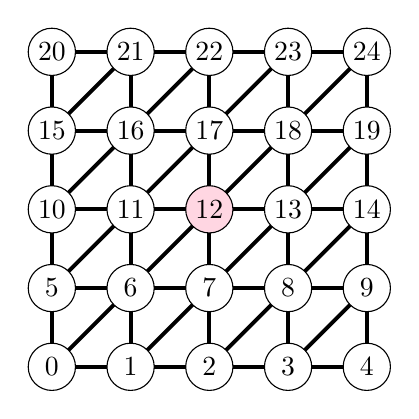
\begin{tikzpicture}[circ/.style = {circle, draw, inner sep=0pt, minimum size=3pt, outer sep=0pt, minimum size=6mm}]
      \pgfmathsetmacro{\lastelementsinrow}{4}
      \foreach \x in {0,...,\lastelementsinrow}
      {
        \foreach \y in {0,...,\lastelementsinrow}
        {
          \pgfmathtruncatemacro{\label}{\y * \lastelementsinrow + \y + \x}
          \ifthenelse{\x=2 \AND \y=2}{\node (\x\y) [circ,fill=r0d] at (\x, \y) {\label}}{\node (\x\y) [circ] at (\x, \y) {\label}};
        }
      }

      \foreach \x in {1,...,\lastelementsinrow}
      {
        \foreach \y in {0,...,\lastelementsinrow}
        {
          \pgfmathtruncatemacro{\px}{\x - 1}
          \draw [line width=0.5mm] (\x\y) -- (\px\y);
        }
      }

      \foreach \x in {0,...,\lastelementsinrow}
      {
        \foreach \y in {1,...,\lastelementsinrow}
        {
          \pgfmathtruncatemacro{\py}{\y - 1}
          \draw [line width=0.5mm] (\x\y) -- (\x\py);
        }
      }

      \foreach \x in {1,...,\lastelementsinrow}
      {
        \foreach \y in {1,...,\lastelementsinrow}
        {
          \pgfmathtruncatemacro{\py}{\y - 1}
          \pgfmathtruncatemacro{\px}{\x - 1}
          \draw [line width=0.5mm] (\x\y) -- (\px\py);
        }
      }
    \end{tikzpicture}
  }
  \qquad
  \subfloat[Matrix]
  {
    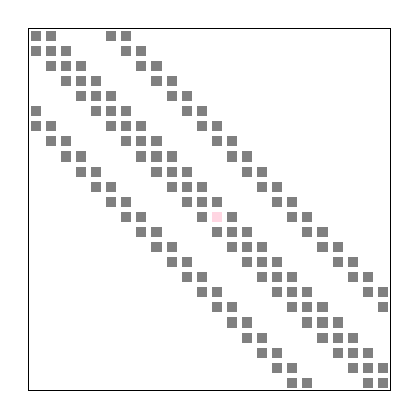
\begin{tikzpicture}
      \pgfmathsetmacro{\size}{4.6}
      \pgfmathsetmacro{\es}{\size/24}
      \pgfmathsetmacro{\pd}{\es/6}
      \pgfmathsetmacro{\ebs}{\es - 2 * \pd}
      \draw (0,0) rectangle ++(\size,\size);

      % Diagonal part
      \foreach \x in {0,...,23}
        \foreach \y in {0,...,23}
         \ifthenelse{\x=\y}
         {
           \ifthenelse{\y=12}
           {
             \fill [r0d] (\es * \x + \pd, \size - \es * \y - \es + \pd) rectangle ++(\ebs, \ebs)
           }
           {
             \fill [gray] (\es * \x + \pd, \size - \es * \y - \es + \pd) rectangle ++(\ebs, \ebs)
           }
         }{};

      % Left part
      \foreach \y in {1,...,23}
       \fill [gray] (\es * \y - \es + \pd, \size - \es * \y - \es + \pd) rectangle ++(\ebs, \ebs);

      % Right part
      \foreach \y in {0,...,22}
       \fill [gray] (\es * \y + \es + \pd, \size - \es * \y - \es + \pd) rectangle ++(\ebs, \ebs);

      % Bottom part
      \foreach \y in {5,...,23}
       \fill [gray] (\es * \y - 5 * \es + \pd, \size - \es * \y - \es + \pd) rectangle ++(\ebs, \ebs);

      % Top part
      \foreach \y in {0,...,18}
       \fill [gray] (\es * \y + 5 * \es + \pd, \size - \es * \y - \es + \pd) rectangle ++(\ebs, \ebs);

      % Diag part
      \foreach \y in {0,...,17}
       \fill [gray] (\es * \y + 6 * \es + \pd, \size - \es * \y - \es + \pd) rectangle ++(\ebs, \ebs);
      \foreach \y in {6,...,23}
       \fill [gray] (\es * \y - 6 * \es + \pd, \size - \es * \y - \es + \pd) rectangle ++(\ebs, \ebs);
    \end{tikzpicture}
  }
  \caption{A simple finite element mesh model}
  \label{fem_to_sparse_matrix}
\end{figure}

\section{Data Structures for Sparse Matrices}
In general, SpMV is limited by memory bandwidth. The storage format used for the sparse matrix defines SpMV algorithm. Each of this
algorithms has it's own granularity, which impacts performance. The primary distinction among sparse matrix representations is the 
sparsity pattern, or the structure of the nonzero entries, for which they are best suited. 

\subsection{CSR}

The \textit{Compressed Sparse Row} (CSR) format is a general sparse matrix format. CSR format consists of three arrays: \textit{row\_ptr},
non-zeroes' \textit{columns} and matrix \textit{values} (fig. \ref{csr_format}). The row's non-zero values are stored consequentially in \textit{values} array. The \textit{row\_ptr} array
is used to divide \textit{values} array into separate rows. It's size is equal to $n\_rows + 1$. The last entry in \textit{row\_ptr} stores number of non-zeroes (NNZ) in the
matrix. That allows fast querying of non-zeroes number in a particular row ($row\_ptr[row+1] - row\_ptr[row]$).
For each non-zero value column index is stored in \textit{columns} array.

\begin{figure}[H]
  \centering
  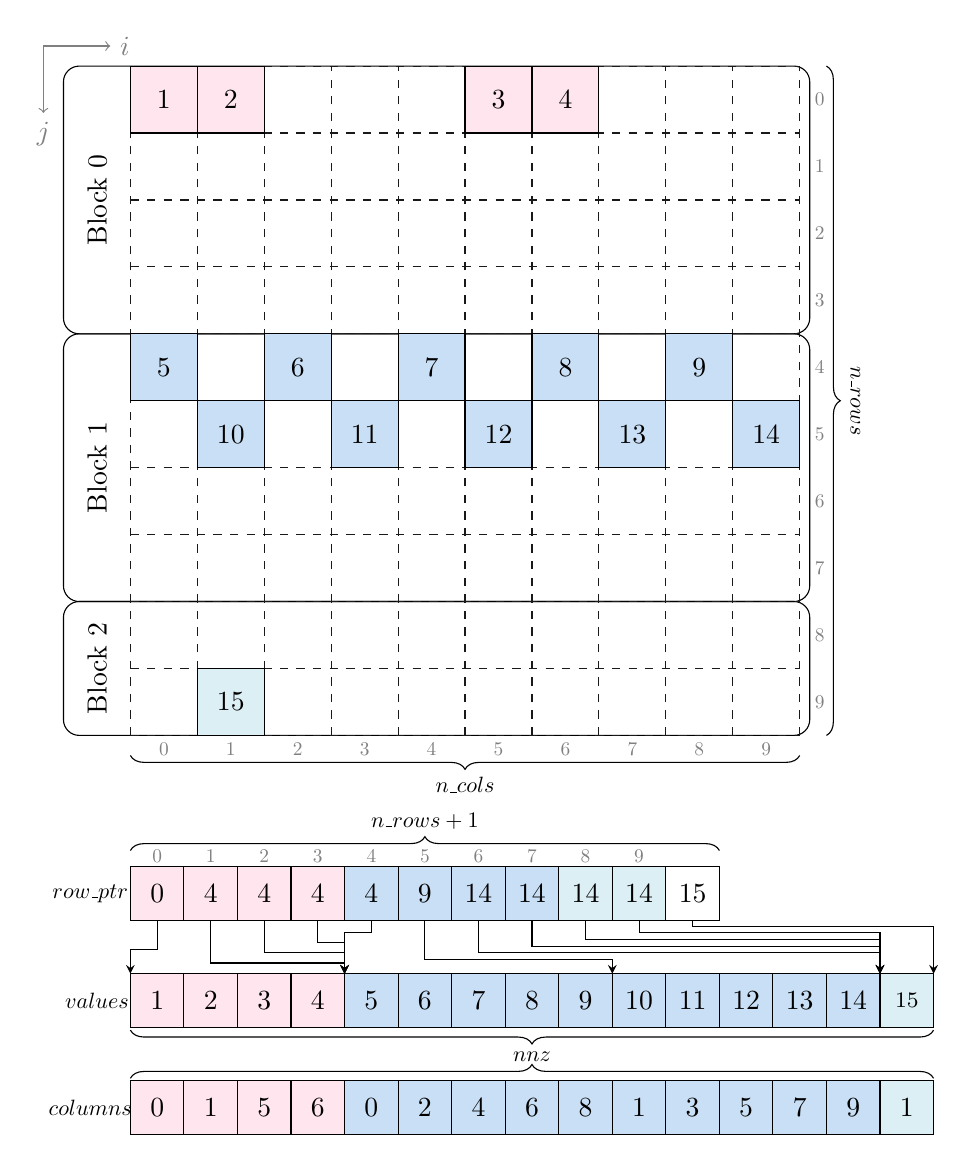
\begin{tikzpicture}[circ/.style = {circle, draw, inner sep=0pt, minimum size=3pt, outer sep=0pt, minimum size=6mm}, scale=0.85]

	\draw[round] (-1.0,0) rectangle (10.15,2.0);
  \draw[round] (-1.0,2.0) rectangle (10.15,6.0);
  \draw[round] (-1.0,6.0) rectangle (10.15,10);

	
  \node[rotate=90] at (-0.5,8){Block 0};
  \node[rotate=90] at (-0.5,4.0) {Block 1};
  \node[rotate=90] at (-0.5,1.)  {Block 2};

  \foreach \y in {0,...,9} {
    \node[scale=0.7,text=gray] at (10.3,10.0 - 1.0*\y - 0.5) {\y};
  }

  \foreach \x in {0,...,9} {
    \node[scale=0.7,text=gray] at (1.0*\x + 0.5,-0.2) {\x};
  }

  \draw[->,gray] (-1.3,10.3) -- (-0.3,10.3) node[right] {$i$};
  \draw[->,gray] (-1.3,10.3) -- (-1.3,9.3) node[below] {$j$};

  % Elements mesh
  \draw[step=1.0,black!90!white,thin,dashed,line width=0.4] (0.0,0.0) grid (10.0,10.0);

  % \draw[round] (-0.15,0) rectangle (10.15,10);

  % Right braces
  \draw [mbrace] (10.4,0.0)  -- (10.4,10.0) node[rightlabel] {$n\_rows$};

  % Bottom braces
  \draw [mbrace] (0.0,-0.3) -- (10,-0.3) node[bottomlabel] {$n\_cols$};

  \edef\esize{1.0}

  % ROW 0
  \edef\elementnum{1}
  \foreach \col in {0,1,5,6} {
    \draw[fill=r0d!60] (\col*\esize,9.0) rectangle (\col*\esize+\esize,10) node[pos=.5] {\elementnum};
    \pgfmathparse{int(\elementnum+1)}
    \xdef\elementnum{\pgfmathresult}
  }

  % ROW 4
  \foreach \col in {0,2,4,6,8} {
    \draw[fill=r1d!60] (\col*\esize,5.0) rectangle (\col*\esize+\esize,6) node[pos=.5] {\elementnum};
    \pgfmathparse{int(\elementnum+1)}
    \xdef\elementnum{\pgfmathresult}
  }

  % ROW 5
  \foreach \col in {1,3,5,7,9} {
    \draw[fill=r1d!60] (\col*\esize,4.0) rectangle (\col*\esize+\esize,5) node[pos=.5] {\elementnum};
    \pgfmathparse{int(\elementnum+1)}
    \xdef\elementnum{\pgfmathresult}
  }

  % ROW 9
  \foreach \col in {1} {
    \draw[fill=r2d!60] (\col*\esize,0.0) rectangle (\col*\esize+\esize,1) node[pos=.5] {\elementnum};
    \pgfmathparse{int(\elementnum+1)}
    \xdef\elementnum{\pgfmathresult}
  }

  % RHS
  \edef\lasty{0}
  \edef\ynum{1}

  % =====================================================
  % ================== Data structures ================== 
  % =====================================================

  % RHS OFFSETS
  \edef\ybot{-1.0}
  \edef\esize{0.8}

  \edef\xnum{0}
  \edef\lastblockoffset{0}
  \edef\lastyoffset{\ybot-\esize*0.8}

  % ROWS NON ZEROS
  \pgfmathparse{\ybot-\esize*2.2}
  \xdef\ybot{\pgfmathresult}

  % MATRIX OFFSETS
  \draw [mbrace] (11 *\esize,\ybot+1.3*\esize)  -- (0*\esize,\ybot+1.3*\esize) node[toplabel] {$n\_rows+1$};

  \node[scale=0.8] at (-0.6,\ybot+\esize/2) {$row\_ptr$};

  \foreach \i in {0,...,9} {
    \node[scale=0.7,text=gray] at (\i * \esize + \esize/2,\ybot+\esize*1.2) {\i};
  }

  \edef\xnum{0}
  \edef\lastblockoffset{0}
  \edef\middlepoint{\ybot-\esize*0.8}

  \foreach \offset in {0,4,4,4,4,9,14,14,14,14,15} {
    \pgfmathparse{\esize*\offset}
    \xdef\lastblockoffset{\pgfmathresult}

    \ifthenelse{\xnum<4}
    { \draw[fill=r0d!60] (\xnum*\esize,\ybot) rectangle (\xnum*\esize+\esize,\ybot+\esize) node[pos=.5] {\offset}; }
    {
      \ifthenelse{\xnum<8}
      { \draw[fill=r1d!60] (\xnum*\esize,\ybot) rectangle (\xnum*\esize+\esize,\ybot+\esize) node[pos=.5] {\offset}; }
      {
        \ifthenelse{\xnum<10}
        { \draw[fill=r2d!60] (\xnum*\esize,\ybot) rectangle (\xnum*\esize+\esize,\ybot+\esize) node[pos=.5] {\offset}; }
        {
          \ifthenelse{\xnum<11}
          { \draw[fill=white] (\xnum*\esize,\ybot) rectangle (\xnum*\esize+\esize,\ybot+\esize) node[pos=.5] {\offset}; }
          { 
          }
        }
      }
    }

    \ifthenelse{\xnum<1}
    { \draw[>=stealth,->] (\xnum*\esize+\esize/2,\ybot) |- (\lastblockoffset,\middlepoint+0.2) -| (\lastblockoffset,\ybot-\esize); }
    {
      \ifthenelse{\xnum<5}
      { \draw[>=stealth,->] (\xnum*\esize+\esize/2,\ybot) |- (\lastblockoffset,\middlepoint+0.15*\xnum-0.15) -| (\lastblockoffset,\ybot-\esize); }
      {
        \ifthenelse{\xnum<15}
        { \draw[>=stealth,->] (\xnum*\esize+\esize/2,\ybot) |- (\lastblockoffset,\middlepoint+0.1*\xnum-0.45) -| (\lastblockoffset,\ybot-\esize); }
        { }
      }
    }

    \pgfmathparse{int(\xnum+1)}
    \xdef\xnum{\pgfmathresult}
  }

  % MATRIX DATA
  \pgfmathparse{\ybot-\esize*2}
  \xdef\ybot{\pgfmathresult}

  \node[scale=0.8] at (-0.5,\ybot+\esize/2) {$values$};

  % Row 0
  \edef\elementnum{1}
  \foreach \i in {0,...,3} {
    \draw[fill=r0d!60]  (\i * \esize,\ybot) rectangle (\i * \esize + \esize,\ybot+\esize) node[pos=0.5] {\elementnum};
    \pgfmathparse{int(\elementnum+1)}
    \xdef\elementnum{\pgfmathresult}
  }

  % Row 4
  \foreach \i in {4,...,8} {
    \draw[fill=r1d!60]  (\i * \esize,\ybot) rectangle (\i * \esize + \esize,\ybot+\esize) node[pos=0.5] {\elementnum};
    \pgfmathparse{int(\elementnum+1)}
    \xdef\elementnum{\pgfmathresult}
  }

  % Row 5
  \foreach \i in {9,...,13} {
    \draw[fill=r1d!60]  (\i * \esize,\ybot) rectangle (\i * \esize + \esize,\ybot+\esize) node[pos=0.5] {\elementnum};
    \pgfmathparse{int(\elementnum+1)}
    \xdef\elementnum{\pgfmathresult}
  }

  % Row 6
  \foreach \i in {14,...,14} {
    \draw[fill=r2d!60]  (\i * \esize,\ybot) rectangle (\i * \esize + \esize,\ybot+\esize) node[pos=0.5] {\footnotesize \elementnum};
    \pgfmathparse{int(\elementnum+1)}
    \xdef\elementnum{\pgfmathresult}
  }

  \draw [mbrace] (0 *\esize,1.01*\ybot)  -- (15*\esize,1.01*\ybot) node[bottomlabel] {$nnz$};
  \draw [mbrace] (15 *\esize,1.01*\ybot-0.9*\esize) -- (0* \esize,1.01*\ybot-0.9*\esize) node[bottomlabel] {};

  \pgfmathparse{\ybot-\esize*2}
  \xdef\ybot{\pgfmathresult}
  \node[scale=0.8] at (-0.6,\ybot+\esize/2) {$columns$};

  \edef\elementnum{0}
  \foreach \i in {0,1,5,6} {
    \draw[fill=r0d!60] (\elementnum * \esize,\ybot) rectangle (\elementnum * \esize + \esize,\ybot+\esize) node[pos=0.5] {\i};
    \pgfmathparse{int(\elementnum+1)}
    \xdef\elementnum{\pgfmathresult}
  }
  \foreach \i in {0,2,4,6,8,1,3,5,7,9} {
    \draw[fill=r1d!60] (\elementnum * \esize,\ybot) rectangle (\elementnum * \esize + \esize,\ybot+\esize) node[pos=0.5] {\i};
    \pgfmathparse{int(\elementnum+1)}
    \xdef\elementnum{\pgfmathresult}
  }
  \foreach \i in {1} {
    \draw[fill=r2d!60] (\elementnum * \esize,\ybot) rectangle (\elementnum * \esize + \esize,\ybot+\esize) node[pos=0.5] {\i};
    \pgfmathparse{int(\elementnum+1)}
    \xdef\elementnum{\pgfmathresult}
  }

  \end{tikzpicture}
  \caption{Example of Compressed Sparse Row (CSR) matrix format}
  \label{csr_format}
\end{figure}

Let's assume for simplicity that there are four threads in each CUDA thread block. General CSR SpMV implementation works at the granularity 
of threads per row (fig. \ref{csr_format_work_distribution}). Hence, the matrix on figure \ref{csr_format} is processed by three thread blocks. 
This implementation is usually referenced as CSR-Scalar (list. \ref{csr_scalar}).

\begin{figure}[H]
  \centering
  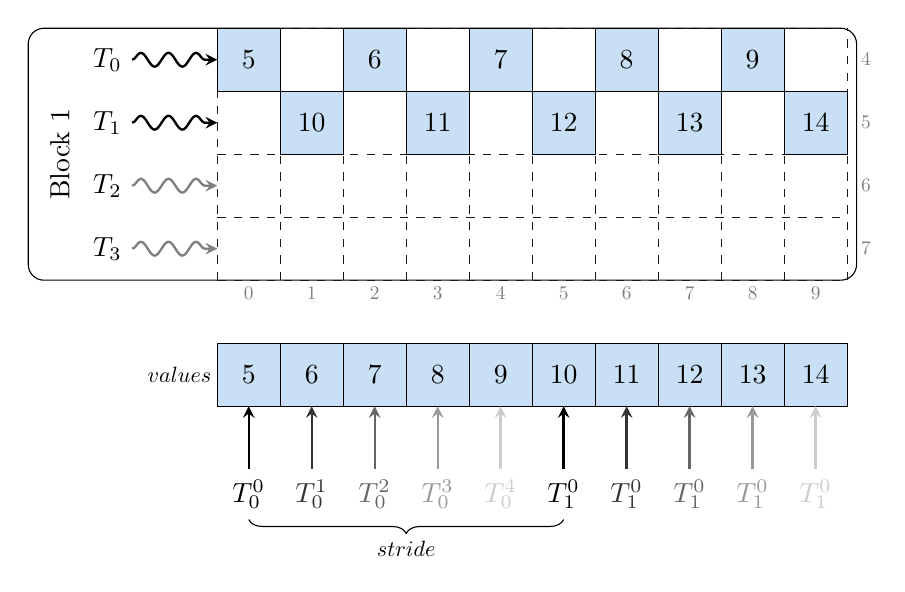
\begin{tikzpicture}[circ/.style = {circle, draw, inner sep=0pt, minimum size=3pt, outer sep=0pt, minimum size=6mm}, scale=0.8]

  \draw[round] (-3.0,2.0) rectangle (10.15,6.0);
  \node[rotate=90] at (-2.5,4.0) {Block 1};

	\draw[draw=black,snake it,line width=0.30mm,>=stealth,->]   (-1.35,5.5) node [anchor=east] {$T_0$} -- (0,5.5);
	\draw[draw=black,snake it,line width=0.30mm,>=stealth,->]   (-1.35,4.5) node [anchor=east] {$T_1$} -- (0,4.5);
	\draw[draw=gray,snake it,line width=0.30mm,>=stealth,->] (-1.35,3.5) node [anchor=east] {$T_2$} -- (0,3.5);
	\draw[draw=gray,snake it,line width=0.30mm,>=stealth,->] (-1.35,2.5) node [anchor=east] {$T_3$} -- (0,2.5);

  \foreach \y in {4,...,7} {
    \node[scale=0.7,text=gray] at (10.3,10.0 - 1.0*\y - 0.5) {\y};
  }

  \foreach \x in {0,...,9} {
    \node[scale=0.7,text=gray] at (1.0*\x + 0.5,1.8) {\x};
  }

  % Elements mesh
  \draw[step=1.0,black!90!white,thin,dashed,line width=0.4] (0.0,2.0) grid (10.0,6.0);

  \edef\esize{1.0}

  % ROW 0
  \edef\elementnum{5}

  % ROW 4
  \foreach \col in {0,2,4,6,8} {
    \draw[fill=r1d!60] (\col*\esize,5.0) rectangle (\col*\esize+\esize,6) node[pos=.5] {\elementnum};
    \pgfmathparse{int(\elementnum+1)}
    \xdef\elementnum{\pgfmathresult}
  }

  % ROW 5
  \foreach \col in {1,3,5,7,9} {
    \draw[fill=r1d!60] (\col*\esize,4.0) rectangle (\col*\esize+\esize,5) node[pos=.5] {\elementnum};
    \pgfmathparse{int(\elementnum+1)}
    \xdef\elementnum{\pgfmathresult}
  }

  % Data access
  \pgfmathparse{2-\esize*2}
  \xdef\ybot{\pgfmathresult}

  \node[scale=0.8] at (-0.6,\ybot+\esize/2) {$values$};

  % Row 0
  \edef\elementnum{5}

  % Row 4
  \foreach \i in {0,...,4} {
    \draw[fill=r1d!60]  (\i * \esize,\ybot) rectangle (\i * \esize + \esize,\ybot+\esize) node[pos=0.5] {\elementnum};
    \pgfmathparse{int(\elementnum+1)}
    \xdef\elementnum{\pgfmathresult}
  }

	\draw[draw=black!100,line width=0.30mm,>=stealth,->] (\esize/2,\ybot-\esize) node [anchor=north] {$T_0^0$} -- (\esize/2,\ybot);
	\draw[draw=black!80,text=black!80,line width=0.30mm,>=stealth,->] (\esize+\esize/2,\ybot-\esize) node [anchor=north] {$T_0^1$} -- (\esize+\esize/2,\ybot);
	\draw[draw=black!60,text=black!60,line width=0.30mm,>=stealth,->] (2*\esize+\esize/2,\ybot-\esize) node [anchor=north] {$T_0^2$} -- (2*\esize+\esize/2,\ybot);
	\draw[draw=black!40,text=black!40,line width=0.30mm,>=stealth,->] (3*\esize+\esize/2,\ybot-\esize) node [anchor=north] {$T_0^3$} -- (3*\esize+\esize/2,\ybot);
	\draw[draw=black!20,text=black!20,line width=0.30mm,>=stealth,->] (4*\esize+\esize/2,\ybot-\esize) node [anchor=north] {$T_0^4$} -- (4*\esize+\esize/2,\ybot);

  % Row 5
  \foreach \i in {5,...,9} {
    \draw[fill=r1d!60]  (\i * \esize,\ybot) rectangle (\i * \esize + \esize,\ybot+\esize) node[pos=0.5] {\elementnum};
    \pgfmathparse{int(\elementnum+1)}
    \xdef\elementnum{\pgfmathresult}
  }

	\draw[draw=black!100,line width=0.30mm,>=stealth,->] (5*\esize+\esize/2,\ybot-\esize) node [anchor=north] {$T_1^0$} -- (5*\esize+\esize/2,\ybot);
	\draw[draw=black!80,text=black!80,line width=0.30mm,>=stealth,->]  (6*\esize+\esize/2,\ybot-\esize) node [anchor=north] {$T_1^0$} -- (6*\esize+\esize/2,\ybot);
	\draw[draw=black!60,text=black!60,line width=0.30mm,>=stealth,->]  (7*\esize+\esize/2,\ybot-\esize) node [anchor=north] {$T_1^0$} -- (7*\esize+\esize/2,\ybot);
	\draw[draw=black!40,text=black!40,line width=0.30mm,>=stealth,->]  (8*\esize+\esize/2,\ybot-\esize) node [anchor=north] {$T_1^0$} -- (8*\esize+\esize/2,\ybot);
	\draw[draw=black!20,text=black!20,line width=0.30mm,>=stealth,->]  (9*\esize+\esize/2,\ybot-\esize) node [anchor=north] {$T_1^0$} -- (9*\esize+\esize/2,\ybot);

  \draw [mbrace] (\esize/2,\ybot-1.8*\esize) -- (5*\esize+\esize/2,\ybot-1.8*\esize) node[bottomlabel] {$stride$};

  \end{tikzpicture}
  \caption{CSR-Scalar block's threads' work distribution}
  \label{csr_format_work_distribution}
\end{figure}

\begin{listing}[H]
\begin{minted}[linenos,tabsize=2]{cuda}
template <typename data_type>
__global__ void csr_spmv_kernel (
		unsigned int n_rows,
		const unsigned int *col_ids,
		const unsigned int *row_ptr,
		const data_type *data,
		const data_type *x,
		data_type *y)
{
	unsigned int row = blockIdx.x * blockDim.x + threadIdx.x;

	if (row < n_rows)
	{
		const int row_start = row_ptr[row];
		const int row_end = row_ptr[row + 1];

		data_type sum = 0;
		for (unsigned int element = row_start; element < row_end; element++)
			sum += data[element] * x[col_ids[element]];
		y[row] = sum;
	}
}
\end{minted}
\caption{Naive SpMV kernel for the CSR-Scalar sparse matrix format}
\label{csr_scalar}
\end{listing}

Presented implementation of CSR SpMV algorithm on the GPU is usually considered very inefficient. The reasons for
inefficiency are load balancing, thread divergence and memory access pattern. As shown on the figure \ref{csr_format_work_distribution} only half
of the block threads has non-zeroes to process. Thus, a single dense row can arbitrarily delay the execution while all
other cores are idle. Moreover, as shown on the figure \ref{csr_format_work_distribution} adjacent threads access matrix values in a strided way. When concurrent threads simultaneously 
access memory addresses that are far apart in physical memory, then there is no chance for the hardware to combine the accesses. Performance
results for naive CSR-Scalar implementation are presented in table \ref{csr_scalar_speedup_table}. 

\begin{table}[H]
	\centering
	\begin{tabular}{ |p{2.6cm}||p{1cm}|p{1cm}|p{1cm}|p{1cm}|  }
	 \hline
		& \multicolumn{2}{|c|}{float} & \multicolumn{2}{|c|}{double}\\
	 \hline
	 NNZ lower limit & avg & max & avg & max  \\
	 \hline
	 10000  & 4.57 & 32.50 & 3.78 & 29.47 \\
	 100000 & 8.90 & 32.50 & 7.24 & 29.47 \\
	 \hline
	\end{tabular}
	\caption{CSR-Scalar speedup}
  \label{csr_scalar_speedup_table}
\end{table}

The speedup distribution is shown in figures \ref{csr_scalar_speedup_float} and \ref{csr_scalar_speedup_double}. To answer the question
how naive described implementation really is I've compared it with the NVIDIA CUDA Sparse Matrix library (cuSPARSE) CSR implementation
(tab. \ref{csr_cusparse_speedup_table}), which has better average speedup (fig. \ref{csr_cusparse_speedup_float} and \ref{csr_cusparse_speedup_double}). 

\begin{table}[H]
	\centering
	\begin{tabular}{ |p{2.6cm}||p{1cm}|p{1cm}|p{1cm}|p{1cm}|  }
	 \hline
		& \multicolumn{2}{|c|}{float} & \multicolumn{2}{|c|}{double}\\
	 \hline
	 NNZ lower limit & avg & max & avg & max  \\
	 \hline
	 10000  & 5.69  & 31.44 & 4.68 & 25.42 \\
	 100000 & 13.62 & 31.44 & 10.65 & 25.42 \\
	 \hline
	\end{tabular}
	\caption{CSR (cuSPARSE) speedup}
  \label{csr_cusparse_speedup_table}
\end{table}

\begin{figure}[H]
\centering
\subfloat[CSR-Scalar speedup (float) \label{csr_scalar_speedup_float}]  {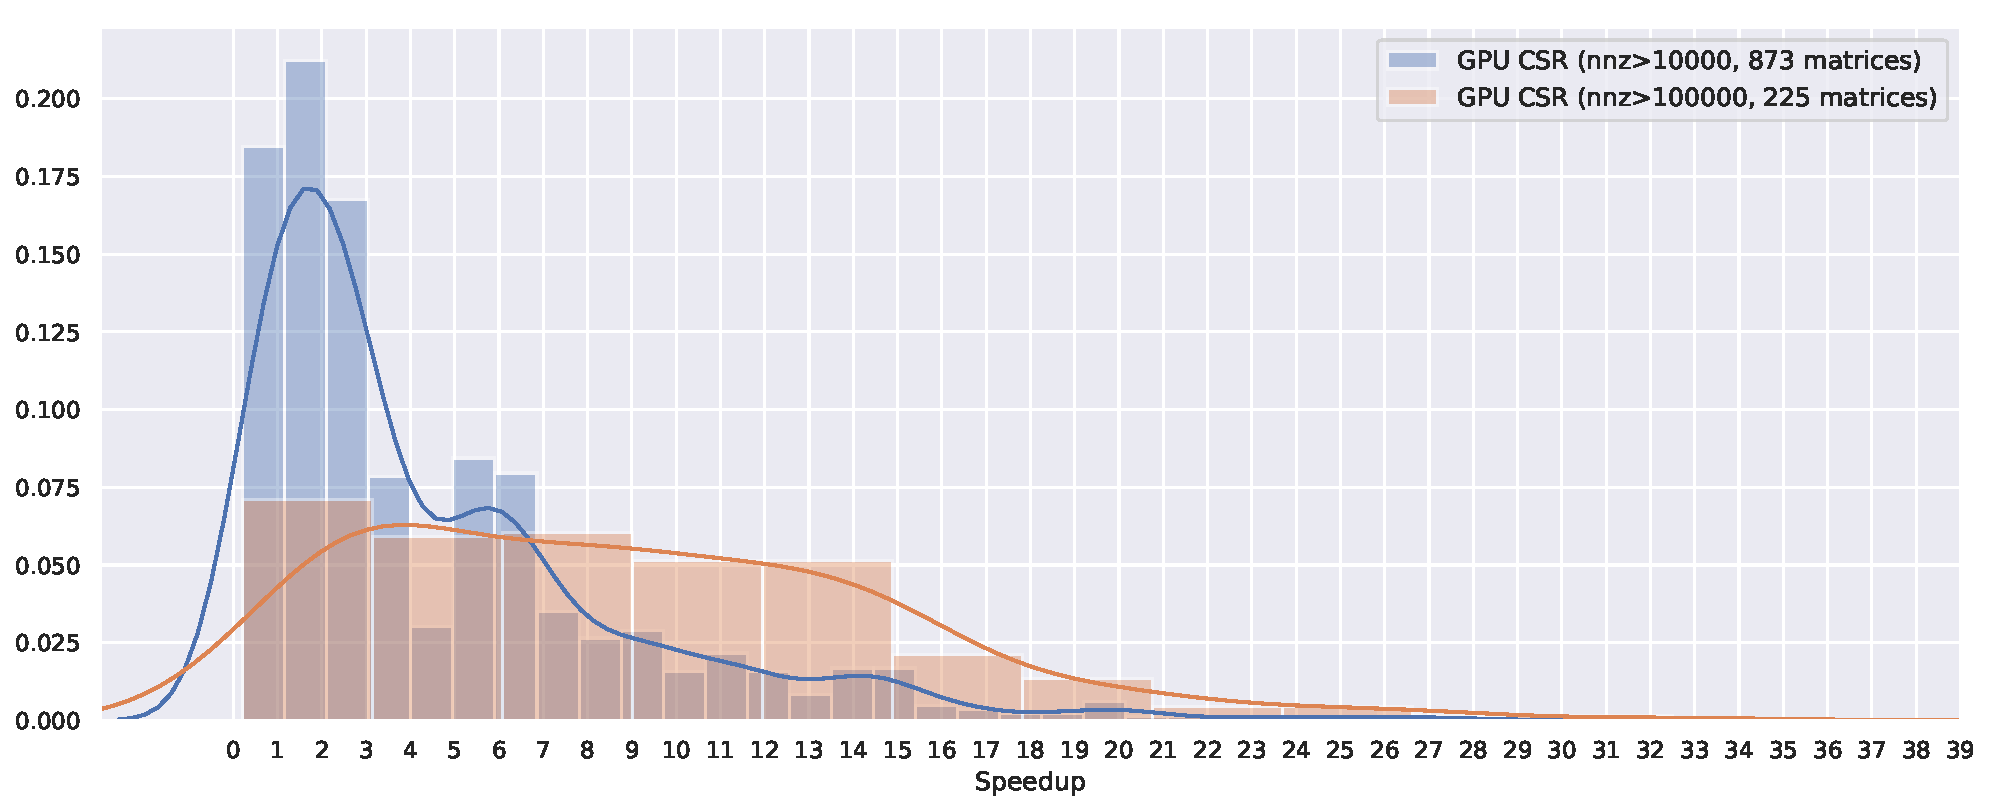
\includegraphics[width=1.0\textwidth]{img/csr_float_dist.pdf}}
\qquad %
\subfloat[CSR-Scalar speedup (double) \label{csr_scalar_speedup_double}] {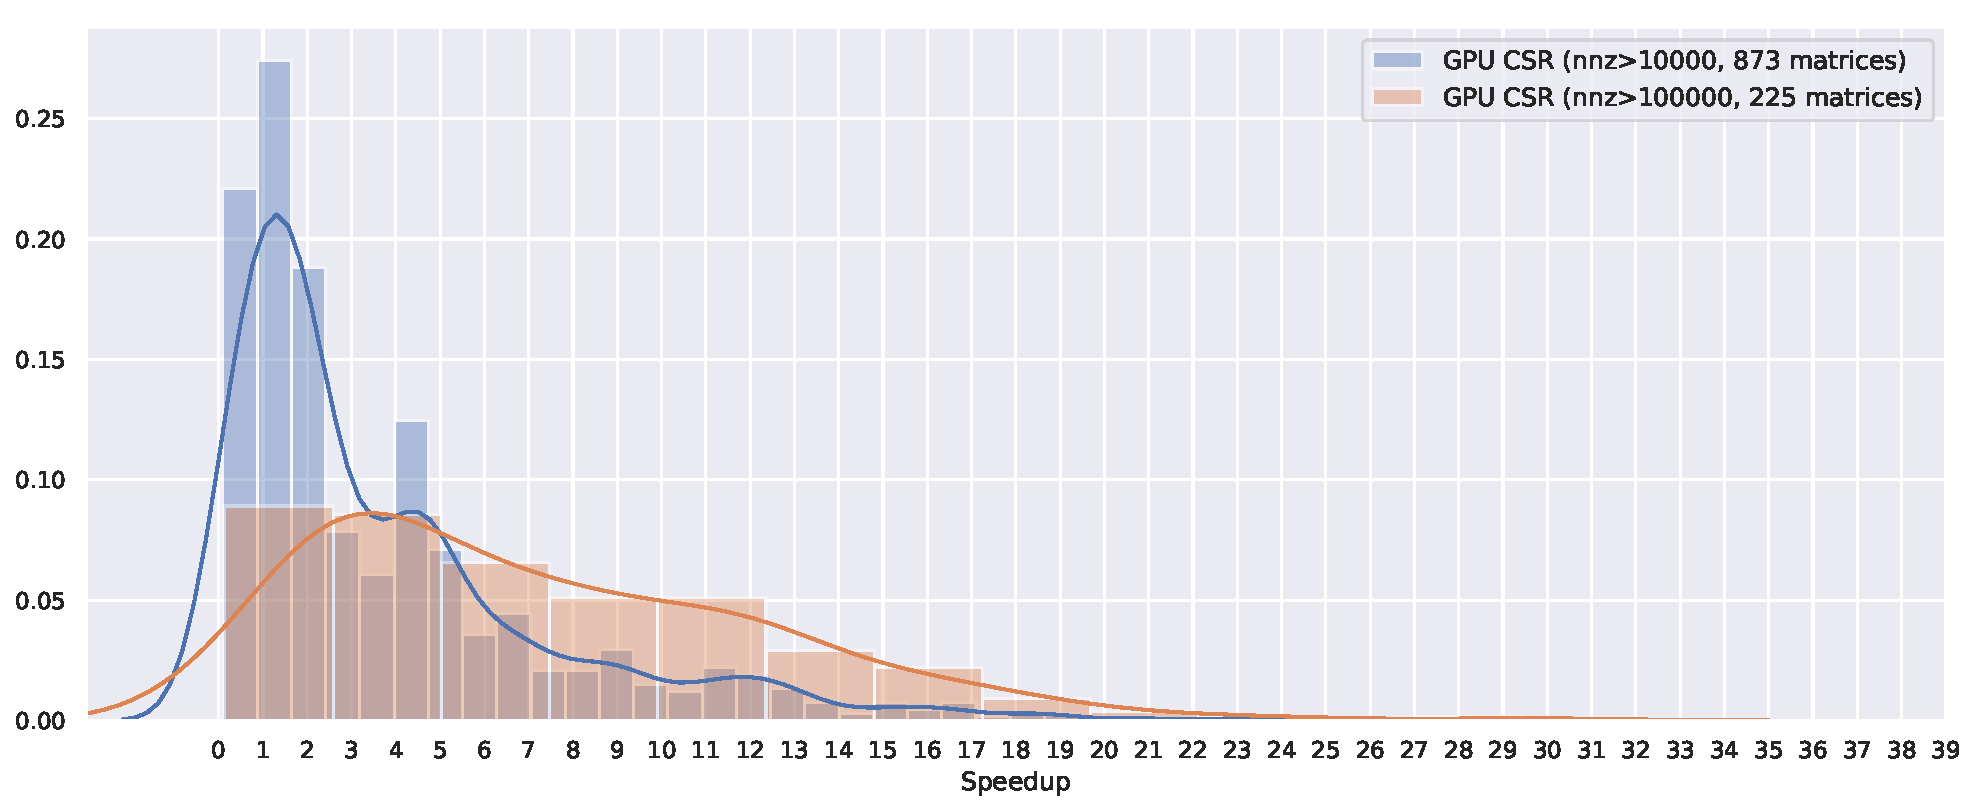
\includegraphics[width=1.0\textwidth]{img/csr_double_dist.pdf}}
\end{figure}

This results shows that there is a room for optimization of CSR SpMV. First possible optimization is to assign warp per row instead of thread.
This algorithm (list. \ref{csr_vector}) is called CSR-Vector. The vector kernel accesses indices and data contiguously, and therefore overcomes 
the principal deficiency of the scalar approach. Unlike the previous CSR implementation, which used one thread per matrix row, this optimization requires
coordination among threads within the same warp. 

\begin{figure}[H]
\centering
\subfloat[CSR cuSPARSE speedup (float) \label{csr_cusparse_speedup_float}]  {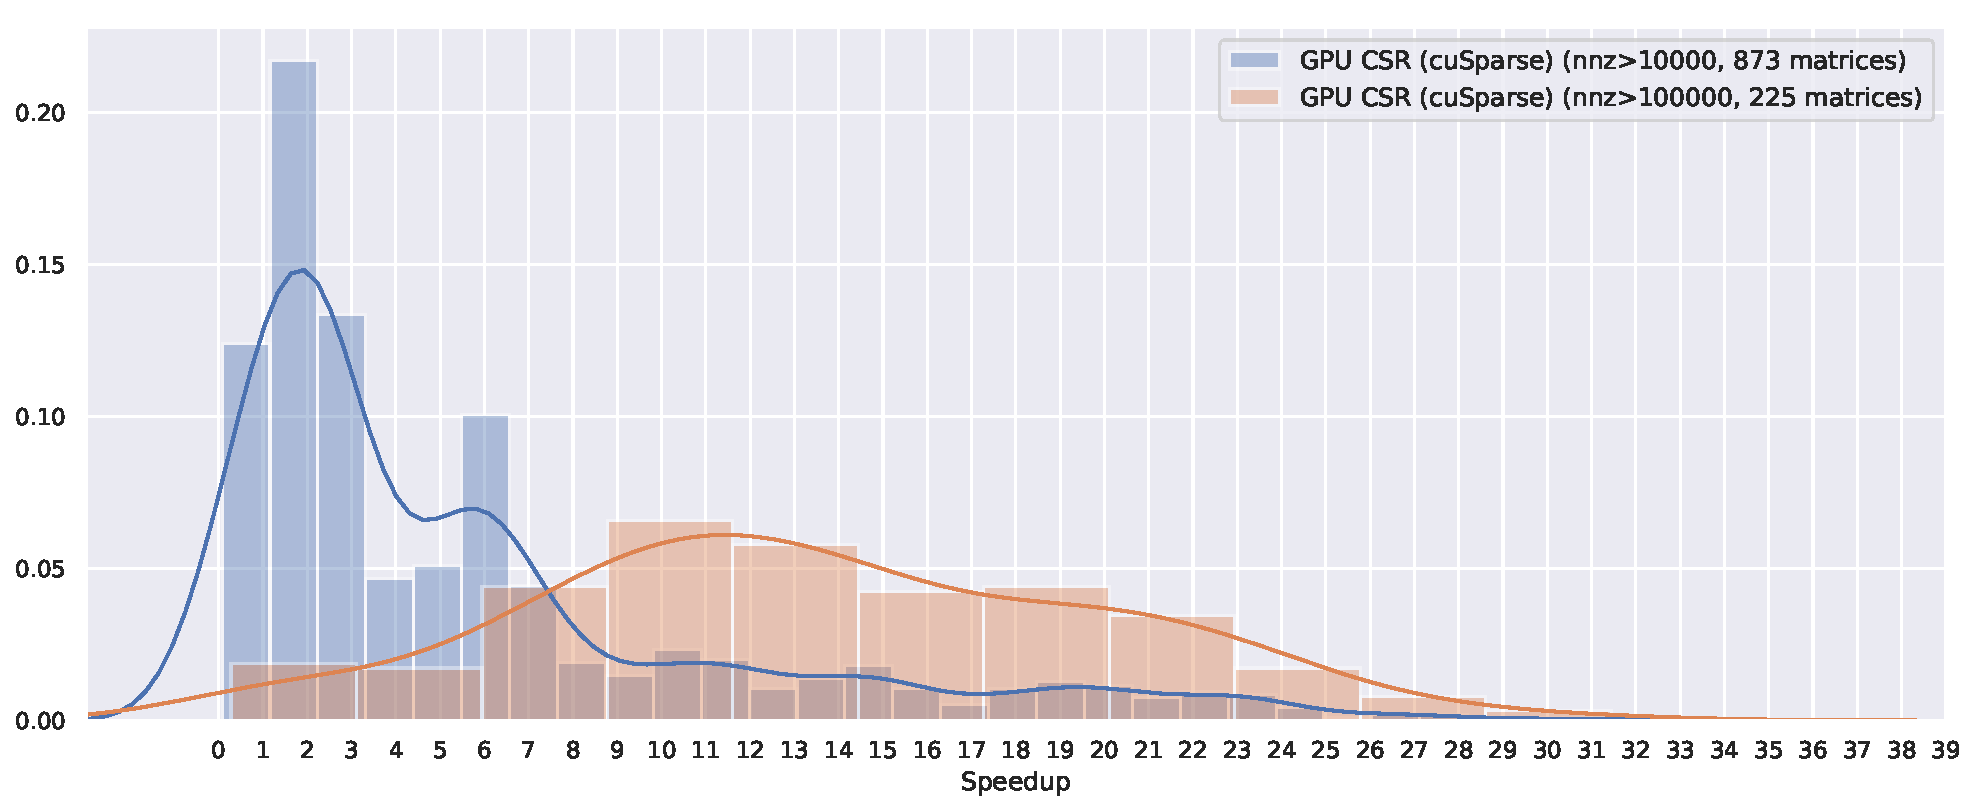
\includegraphics[width=1.0\textwidth]{img/csr_cusparse_float_dist.pdf}}
\qquad %
\subfloat[CSR cuSPARSE speedup (double) \label{csr_cusparse_speedup_double}] {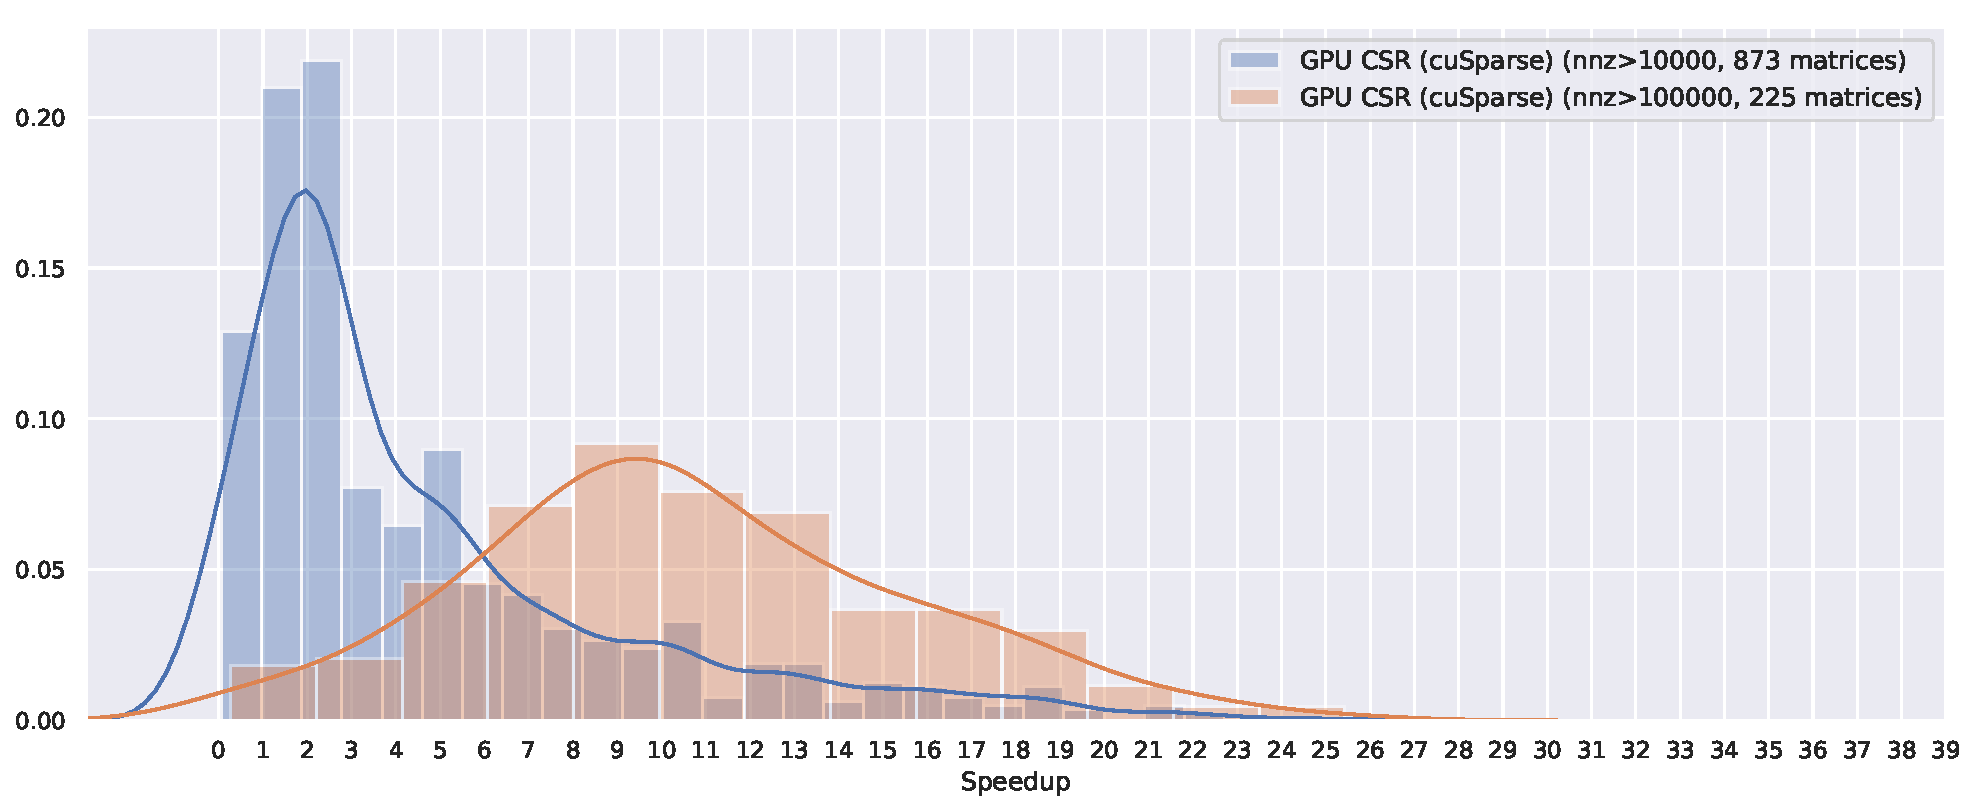
\includegraphics[width=1.0\textwidth]{img/csr_cusparse_double_dist.pdf}}
\end{figure}

In case of CSR-Vector reduction might be implemented using warp-level primitives (list. \ref{warp_reduce}). In that case the data 
exchange is performed between registers, and more efficient than going through shared memory, which requires a load, 
a store and an extra register to hold the address.

\begin{listing}[H]
\begin{minted}[linenos,tabsize=2]{cuda}
template <class T>
__device__ T warp_reduce (T val)
{
  for (int offset = warpSize / 2; offset > 0; offset /= 2)
    val += __shfl_down_sync (FULL_WARP_MASK, val, offset);

  return val;
}
\end{minted}
\caption{Warp reduction}
\label{warp_reduce}
\end{listing}

\begin{listing}[H]
\begin{minted}[linenos,tabsize=2]{cuda}
template <typename data_type>
__global__ void csr_spmv_vector_kernel (
    unsigned int n_rows,
    const unsigned int *col_ids,
    const unsigned int *row_ptr,
    const data_type *data,
    const data_type *x,
    data_type *y)
{
  const unsigned int thread_id = blockIdx.x * blockDim.x + threadIdx.x;
  const unsigned int warp_id = thread_id / 32;
  const unsigned int lane = thread_id % 32;

  const unsigned int row = warp_id; ///< One warp per row

  data_type sum = 0;
  if (row < n_rows)
  {
    const unsigned int row_start = row_ptr[row];
    const unsigned int row_end = row_ptr[row + 1];

    for (unsigned int element = row_start + lane; element < row_end; element += 32)
      sum += data[element] * x[col_ids[element]];
  }

  sum = warp_reduce (sum);

  if (lane == 0 && row < n_rows)
    y[row] = sum;
}
\end{minted}
\caption{SpMV kernel for the CSR sparse matrix format (vector)}
\label{csr_vector}
\end{listing}

\subsection{COO}

\subsection{ELL}

\subsection{Hybrid}


\section{Conclusion}
Write your conclusion here.

\end{document}
